\documentclass[journal]{vgtc}                % final (journal style)
%\documentclass[review,journal]{vgtc}         % review (journal style)
%\documentclass[widereview]{vgtc}             % wide-spaced review
%\documentclass[preprint,journal]{vgtc}       % preprint (journal style)

%% Uncomment one of the lines above depending on where your paper is
%% in the conference process. ``review'' and ``widereview'' are for review
%% submission, ``preprint'' is for pre-publication, and the final version
%% doesn't use a specific qualifier.

%% Please use one of the ``review'' options in combination with the
%% assigned online id (see below) ONLY if your paper uses a double blind
%% review process. Some conferences, like IEEE Vis and InfoVis, have NOT
%% in the past.

%% Please note that the use of figures other than the optional teaser is not permitted on the first page
%% of the journal version.  Figures should begin on the second page and be
%% in CMYK or Grey scale format, otherwise, colour shifting may occur
%% during the printing process.  Papers submitted with figures other than the optional teaser on the
%% first page will be refused. Also, the teaser figure should only have the
%% width of the abstract as the template enforces it.

%% These few lines make a distinction between latex and pdflatex calls and they
%% bring in essential packages for graphics and font handling.
%% Note that due to the \DeclareGraphicsExtensions{} call it is no longer necessary
%% to provide the the path and extension of a graphics file:
%% 
\includegraphics{diamondrule} is completely sufficient.
%%
\ifpdf%                                % if we use pdflatex
  \pdfoutput=1\relax                   % create PDFs from pdfLaTeX
  \pdfcompresslevel=9                  % PDF Compression
  \pdfoptionpdfminorversion=7          % create PDF 1.7
  \ExecuteOptions{pdftex}
  \usepackage{graphicx}                % allow us to embed graphics files
  \DeclareGraphicsExtensions{.pdf,.png,.jpg,.jpeg} % for pdflatex we expect .pdf, .png, or .jpg files
\else%                                 % else we use pure latex
  \ExecuteOptions{dvips}
  \usepackage{graphicx}                % allow us to embed graphics files
  \DeclareGraphicsExtensions{.eps}     % for pure latex we expect eps files
\fi%

%% it is recomended to use ``\autoref{sec:bla}'' instead of ``Fig.~\ref{sec:bla}''
\graphicspath{{gfx/}{./}} % where to search for the images

\usepackage{microtype}                 % use micro-typography (slightly more compact, better to read)
\PassOptionsToPackage{warn}{textcomp}  % to address font issues with \textrightarrow
\usepackage{textcomp}                  % use better special symbols
\usepackage{mathptmx}                  % use matching math font
\usepackage{times}                     % we use Times as the main font
\renewcommand*\ttdefault{txtt}         % a nicer typewriter font
\usepackage{cite}                      % needed to automatically sort the references
\usepackage{tabu}                      % only used for the table example
\usepackage{booktabs}                  % only used for the table example
\usepackage{makecell}
\usepackage{multirow}
\usepackage[export]{adjustbox}
\usepackage{subfig}

%% We encourage the use of mathptmx for consistent usage of times font
%% throughout the proceedings. However, if you encounter conflicts
%% with other math-related packages, you may want to disable it.

%% In preprint mode you may define your own headline.
%\preprinttext{To appear in IEEE Transactions on Visualization and Computer Graphics.}

%% If you are submitting a paper to a conference for review with a double
%% blind reviewing process, please replace the value ``0'' below with your
%% OnlineID. Otherwise, you may safely leave it at ``0''.
\onlineid{0}

%% declare the category of your paper, only shown in review mode
\vgtccategory{Research}
%% please declare the paper type of your paper to help reviewers, only shown in review mode
%% choices:
%% * algorithm/technique
%% * application/design study
%% * evaluation
%% * system
%% * theory/model
\vgtcpapertype{theory/model}

%% Paper title.
% James' title suggestions
% - Reproducing 'Graphical Perception' with CNNs
% - 
\title{Supplemental Material for\\Evaluating `Graphical Perception' with CNNs}

%% This is how authors are specified in the journal style

%% indicate IEEE Member or Student Member in form indicated below
%\author{Daniel Haehn, \textit{Member, IEEE}, James Tompkin, and Hanspeter Pfister}
\author{Daniel Haehn, James Tompkin, and Hanspeter Pfister}
\authorfooter{
%% insert punctuation at end of each item
\item Daniel Haehn, and Hanspeter Pfister are with Harvard University. \\
E-mail: \{haehn,pfister\}@seas.harvard.edu.
%
\item James Tompkin is with Brown University. \\E-mail: james\_tompkin@brown.edu.
}

%other entries to be set up for journal
\shortauthortitle{Haehn \MakeLowercase{\textit{et al.}}: Evaluating `Graphical Perception' with CNNs}
%\shortauthortitle{Firstauthor \MakeLowercase{\textit{et al.}}: Paper Title}


%% ACM Computing Classification System (CCS). 
%% See <http://www.acm.org/class/1998/> for details.
%% The ``\CCScat'' command takes four arguments.

%\CCScatlist{ % not used in journal version
% \CCScat{K.6.1}{Management of Computing and Information Systems}%
%{Project and People Management}{Life Cycle};
% \CCScat{K.7.m}{The Computing Profession}{Miscellaneous}{Ethics}
%}

%% Uncomment below to include a teaser figure.
%\teaser{
%  \centering
%\par{\\~\\~\\~\\}
%}

%% Uncomment below to disable the manuscript note
\renewcommand{\manuscriptnotetxt}{}

%% Copyright space is enabled by default as required by guidelines.
%% It is disabled by the 'review' option or via the following command:
% \nocopyrightspace

%\vgtcinsertpkg

%%%%%%%%%%%%%%%%%%%%%%%%%%%%%%%%%%%%%%%%%%%%%%%%%%%%%%%%%%%%%%%%
%%%%%%%%%%%%%%%%%%%%%% START OF THE PAPER %%%%%%%%%%%%%%%%%%%%%%
%%%%%%%%%%%%%%%%%%%%%%%%%%%%%%%%%%%%%%%%%%%%%%%%%%%%%%%%%%%%%%%%%

\begin{document}
\maketitle

We present several plots which contain complete results for the elementary perceptual task experiment, for which, given the number of experiments, the main paper presented only a selection. We report MLAE for all added parameters to the stimuli, rather than just the most complex parameterization as in the main paper (Figures~\ref{fig:epc_mlae} and \ref{fig:epc_mlae_boxplots}). From this, we see that performance is largely equal across parameters, showing that most networks have sufficient capacity for the given parameterizations.

We also report complete results for the cross-network variability experiment on the elementary perceptual task experiment (Figure \ref{fig:cross_network}). As in the main paper, this shows that our networks are not able to generalize to additional translation or stroke width parameters without representative training data.

Further, we show how the errors for each network are distributed, across elementary perceptual tasks and across different cross-validation splits (Figure~\ref{fig:errors}). Most errors are approximately normally distributed, though our CNN with less parameters (LeNet) and our MLP often have errors which are farther from a normal distribution, and show structure.

\section{Experiment: Anti-aliasing}
We also include an experimental result showing that, for our stimuli, adding anti-aliasing to the line generation was not important to the tested CNNs (Figure~\ref{fig:aa}).

\begin{figure}[h]
\centering
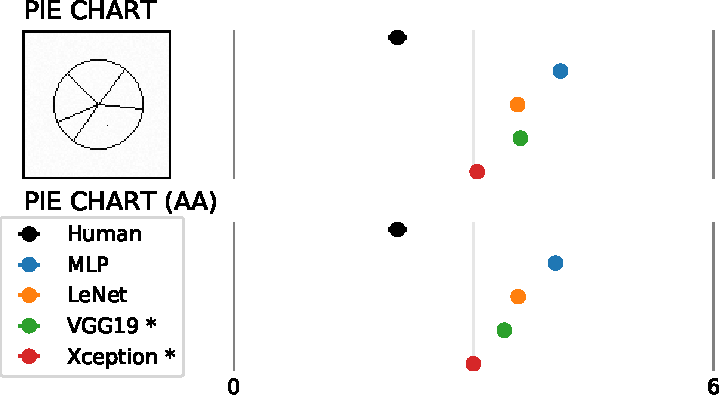
\includegraphics[width=\linewidth]{../gfx/figure3_mlae_better_all_AA.pdf}
\caption{\textbf{Anti-aliasing.} We test whether anti-aliasing effects the performance of our networks on pie charts by measuring MLAE. The difference is not statistically significant ($F(1,30)=0.341,p>0.5$).}
\label{fig:aa}
\end{figure}
\vfill\null
\section{Experiment: Noise}
For all our experiments, we add subtle $5\%$ noise to every pixel to enhance variability. We did not observe a significant effect on regression performance when comparing the weber-fechner's law experiment with and without noise averaged over 4 runs (Figure~\ref{fig:noise}). However, the variability of our stimuli increases.

\begin{figure}[th]
\centering
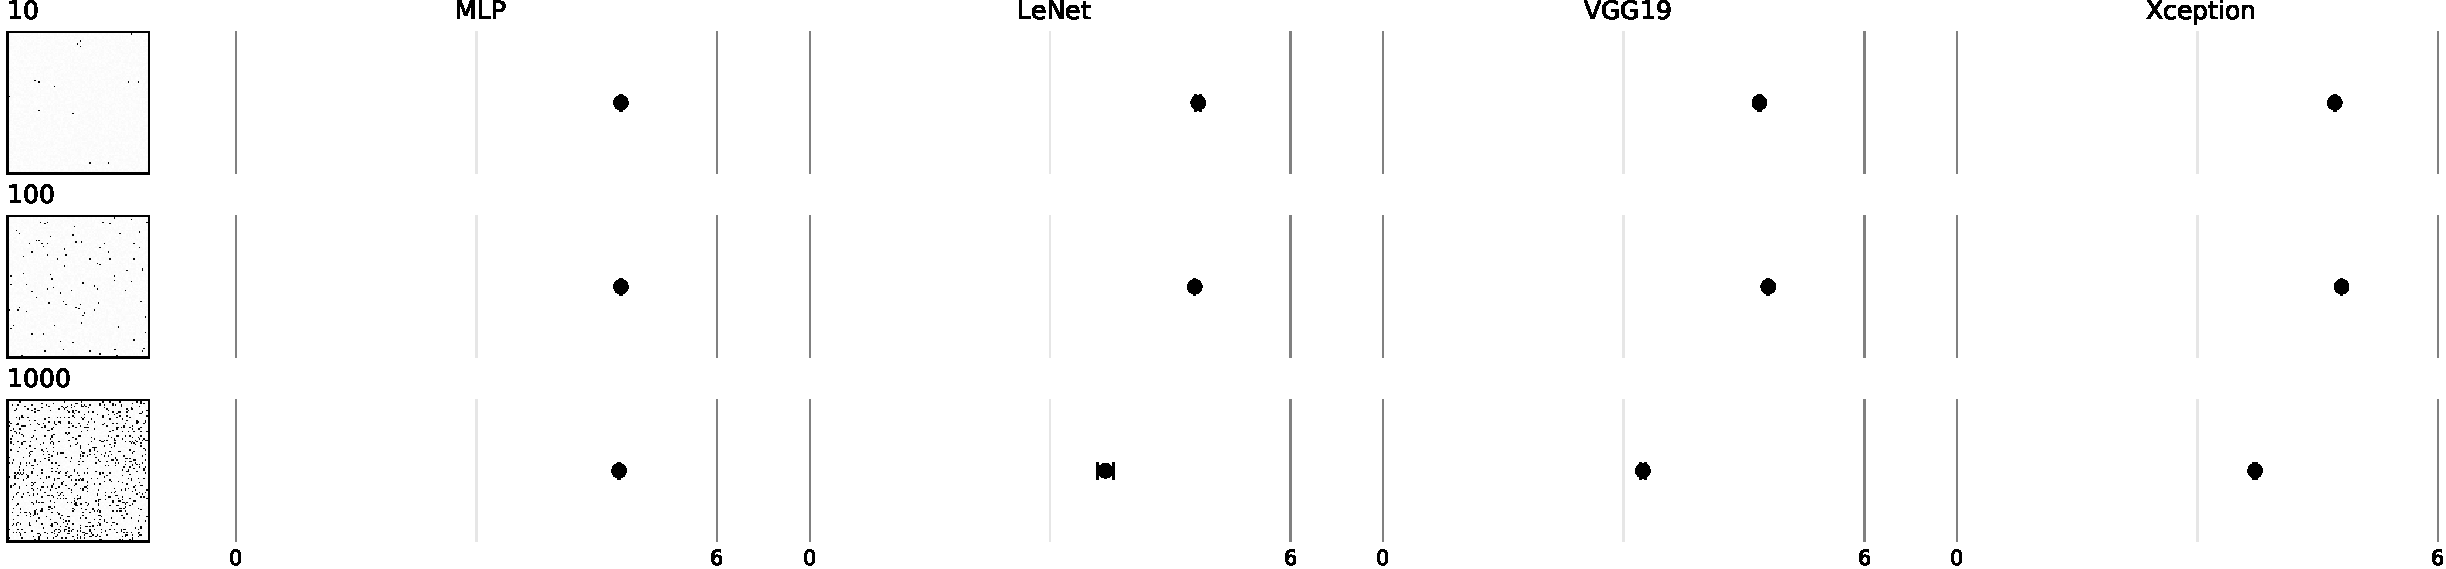
\includegraphics[width=.8\linewidth]{../gfx/weber_mlae_no_noise.pdf}
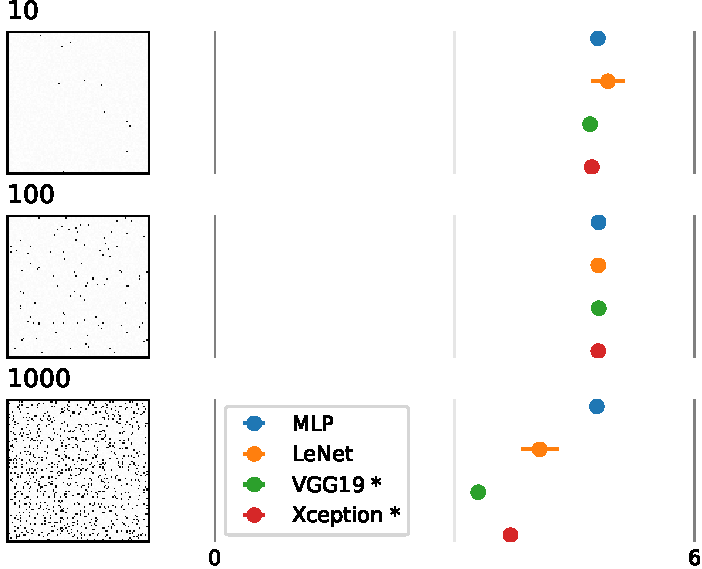
\includegraphics[width=.8\linewidth]{../gfx/weber_mlae_noise.pdf}
\caption{\textbf{Noise.} We test whether noise (top: off, bottom: on) effects the performance of our networks on the weber-fechner's law experiment by measuring MLAE. With noise, $MLAE=4.511$ ($SD=0.512$) and without noise $MLAE=4.491$ ($SD=0.543$). The difference is not statistically significant ($F(1,22)=0.008,p>0.5$).}
\label{fig:noise}
\end{figure}


%% The ``\maketitle'' command must be the first command after the
%% ``\begin{document}'' command. It prepares and prints the title block.

%% the only exception to this rule is the \firstsection command

\begin{figure*}[p]
	\centering
		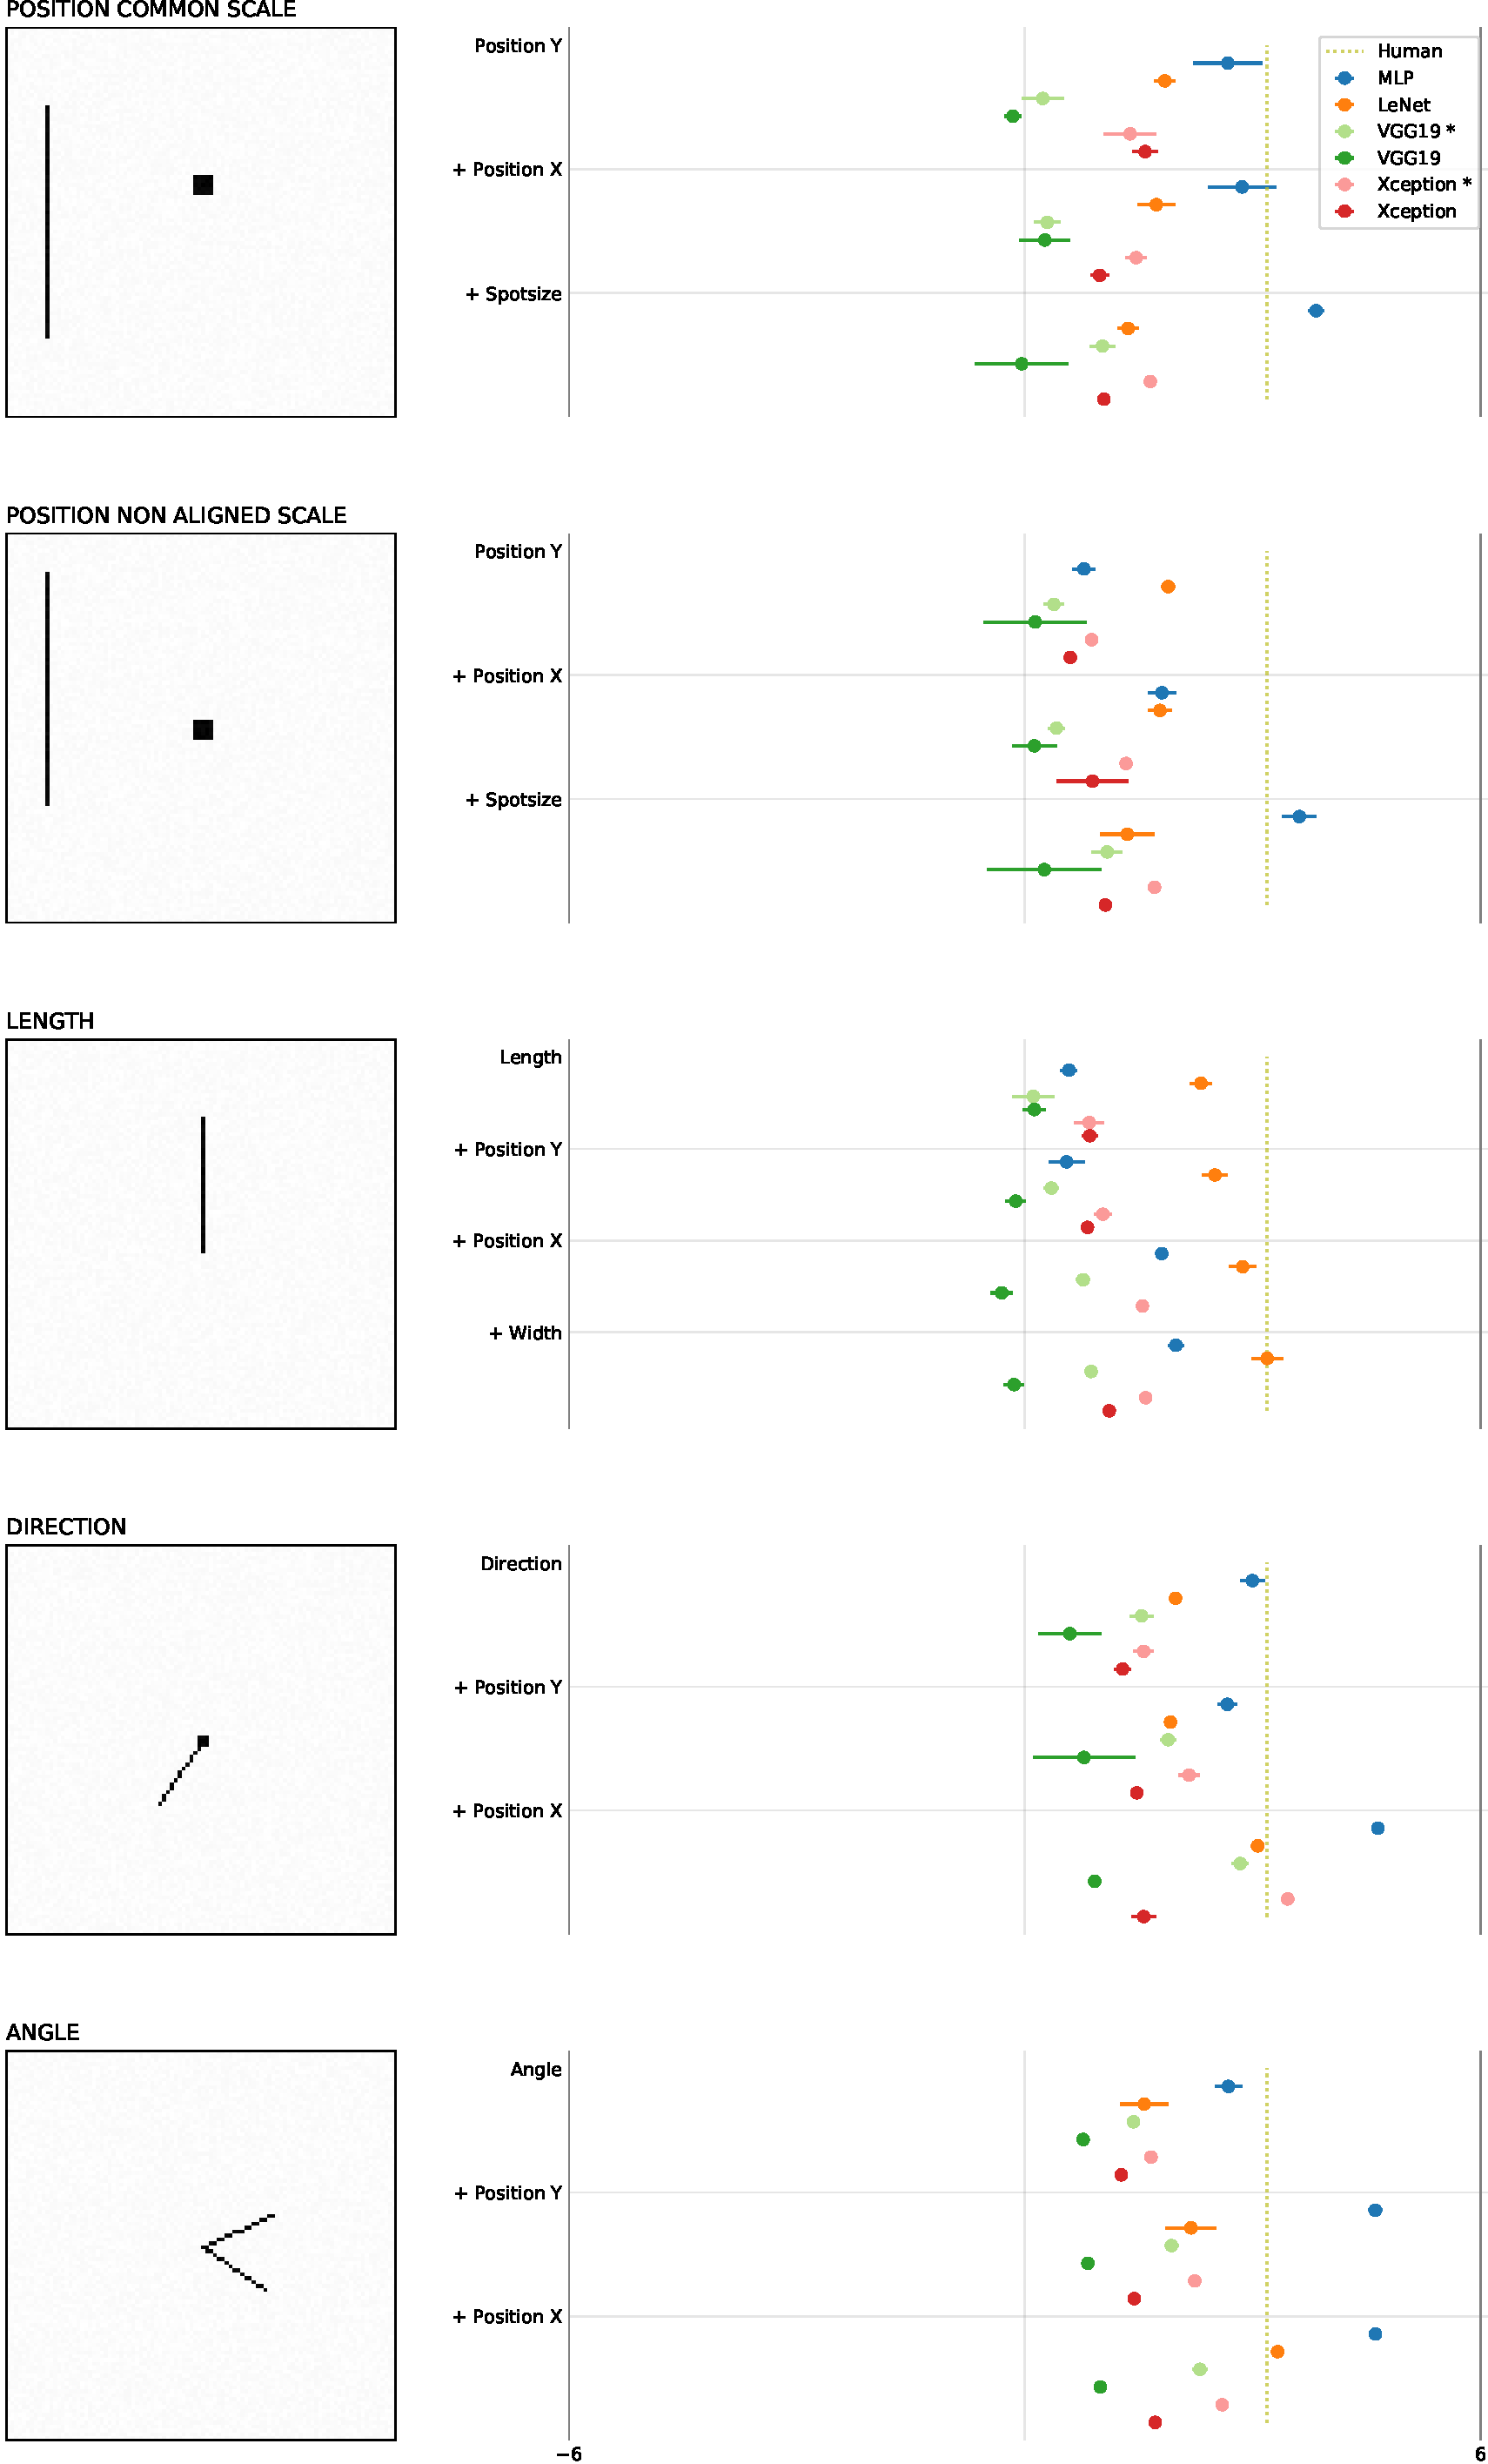
\includegraphics[width=.48\linewidth]{../gfx/figure1_slim_left.pdf}
	  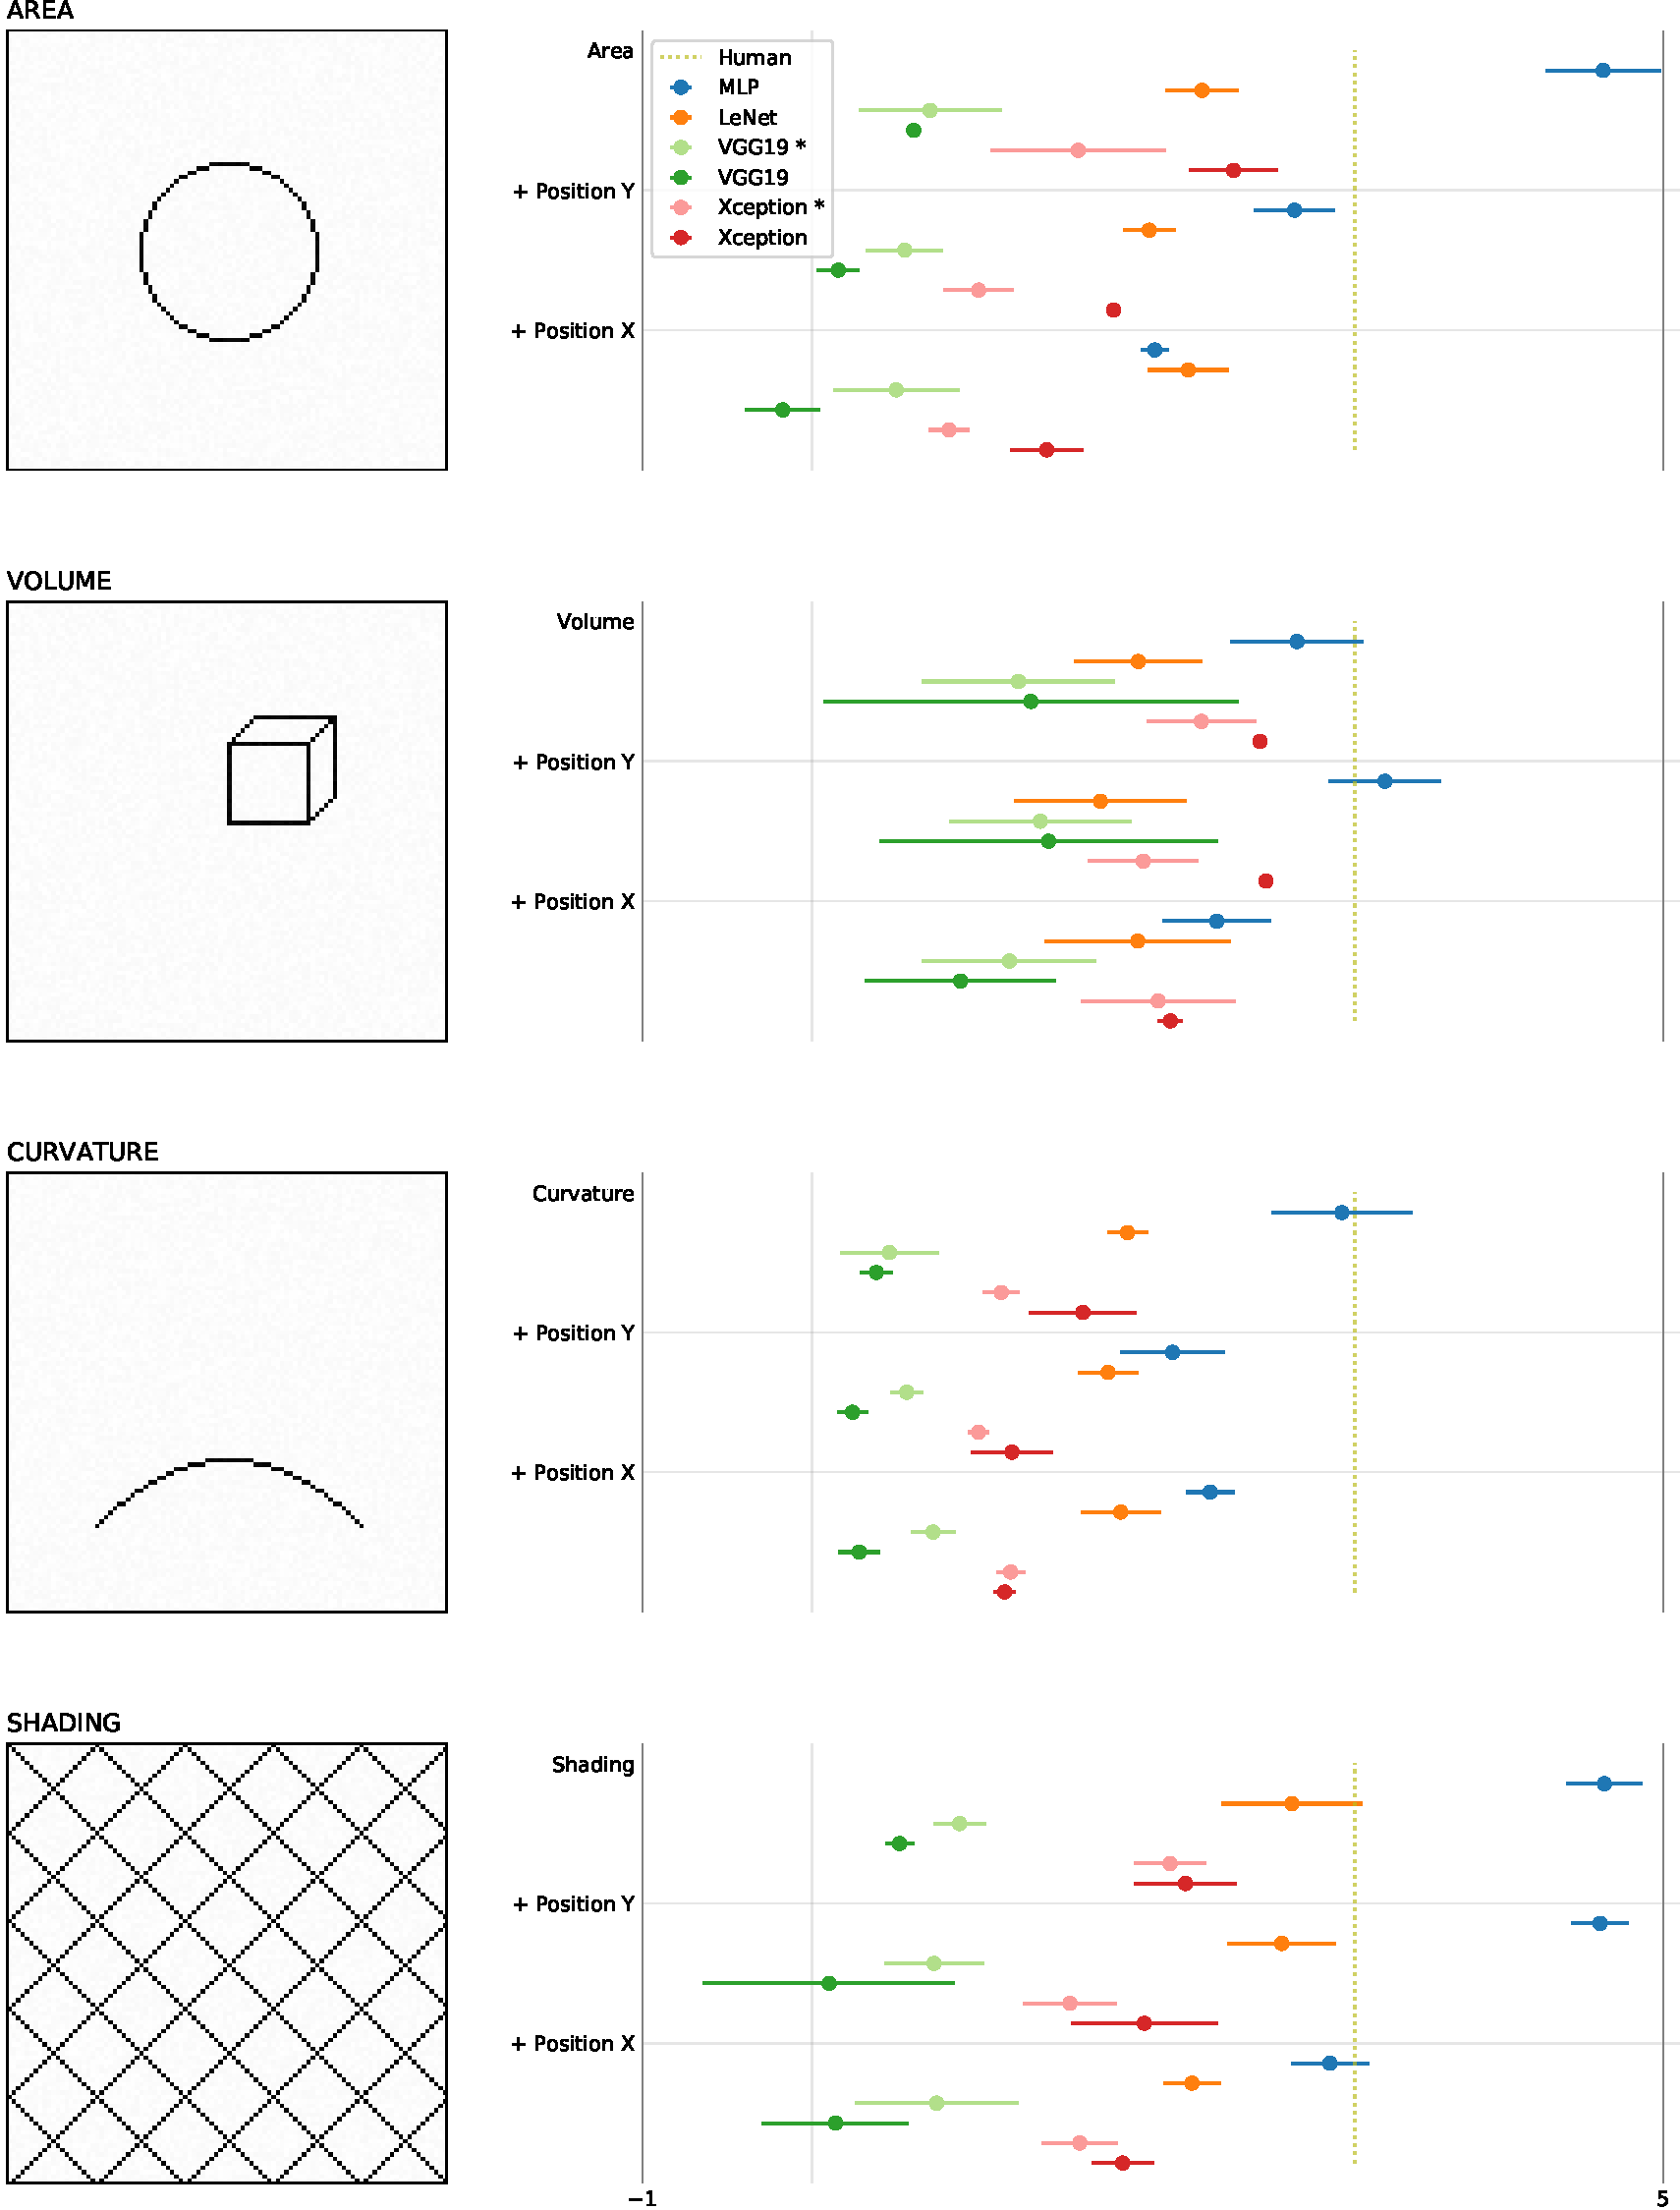
\includegraphics[width=.48\linewidth]{../gfx/figure1_slim_right.pdf}
  \caption{\textbf{Elementary perceptual tasks.} Midmean logistic absolute errors (MLAE) for all generated stimuli and across all networks. The * indicates networks which use ImageNet weights instead of bein trained from scratch.}
	\label{fig:epc_mlae}
\end{figure*}

\begin{figure*}[p]
	\centering
		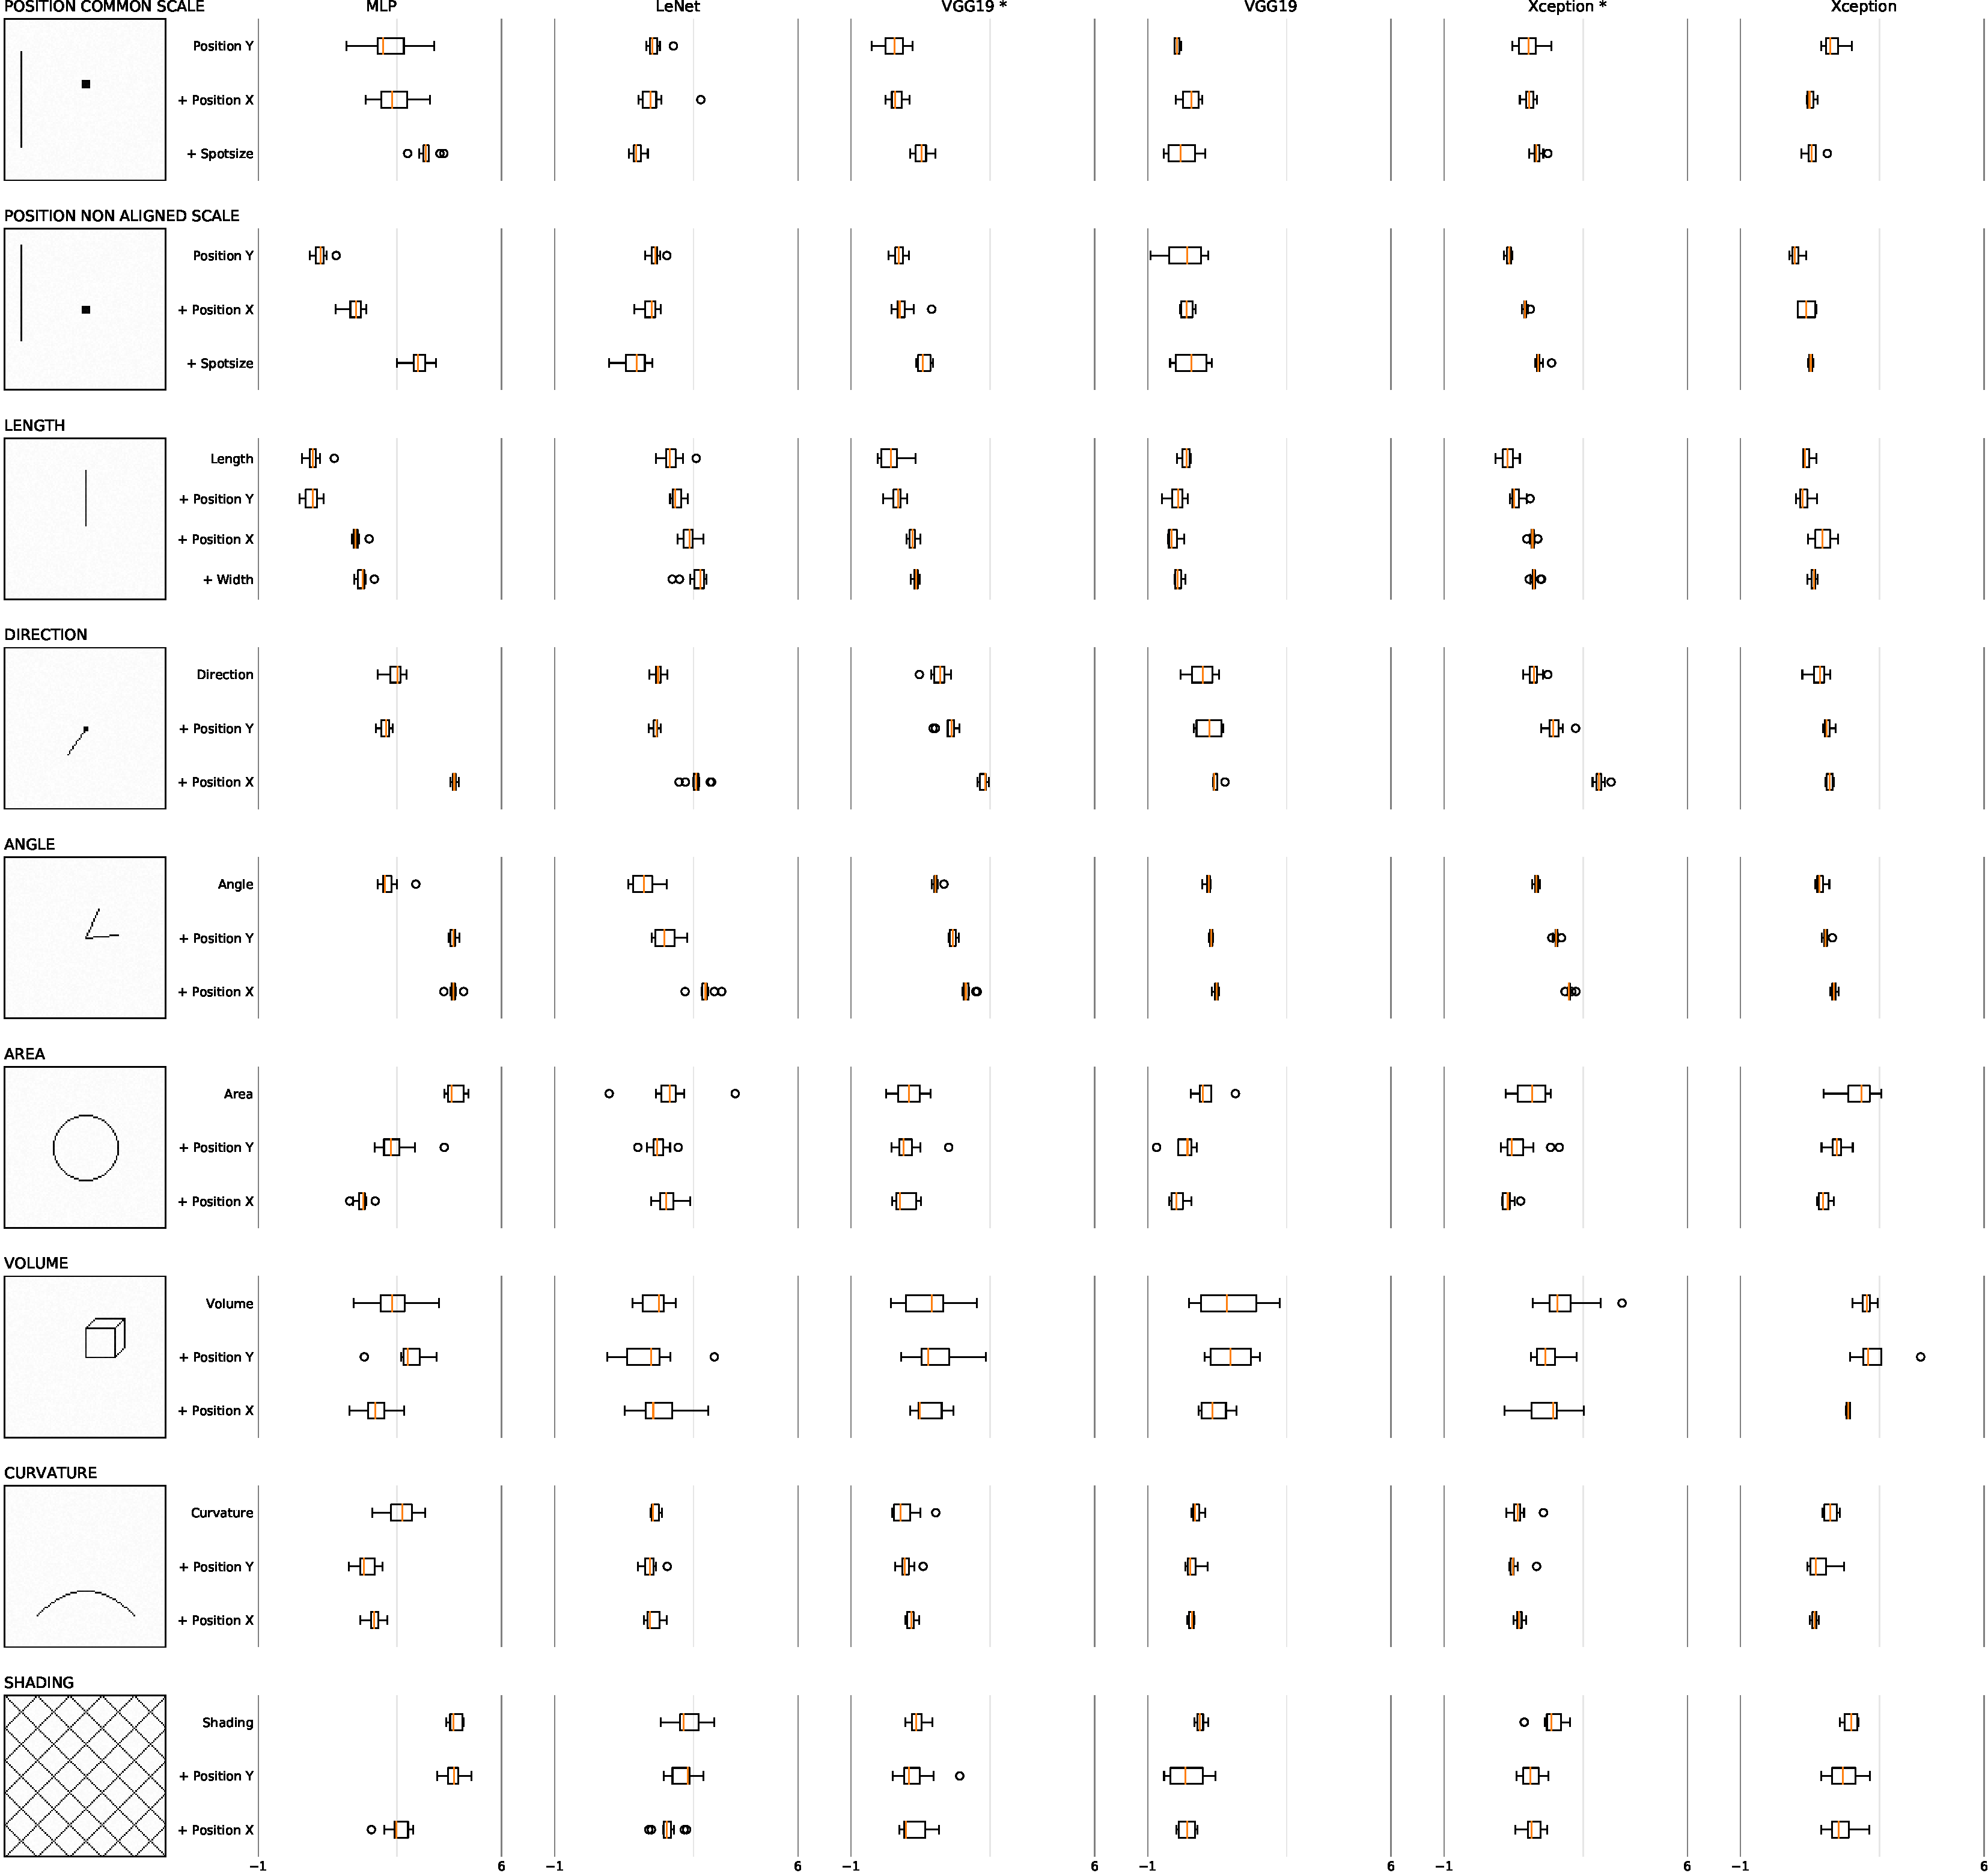
\includegraphics[width=\linewidth]{../gfx/figure1_boxplot_new.pdf}
  \caption{\textbf{Elementary perceptual tasks.} Midmean logistic absolute errors (MLAE) visualized as box plots.}
	\label{fig:epc_mlae_boxplots}
\end{figure*}

\begin{figure*}[p]
	\centering
	  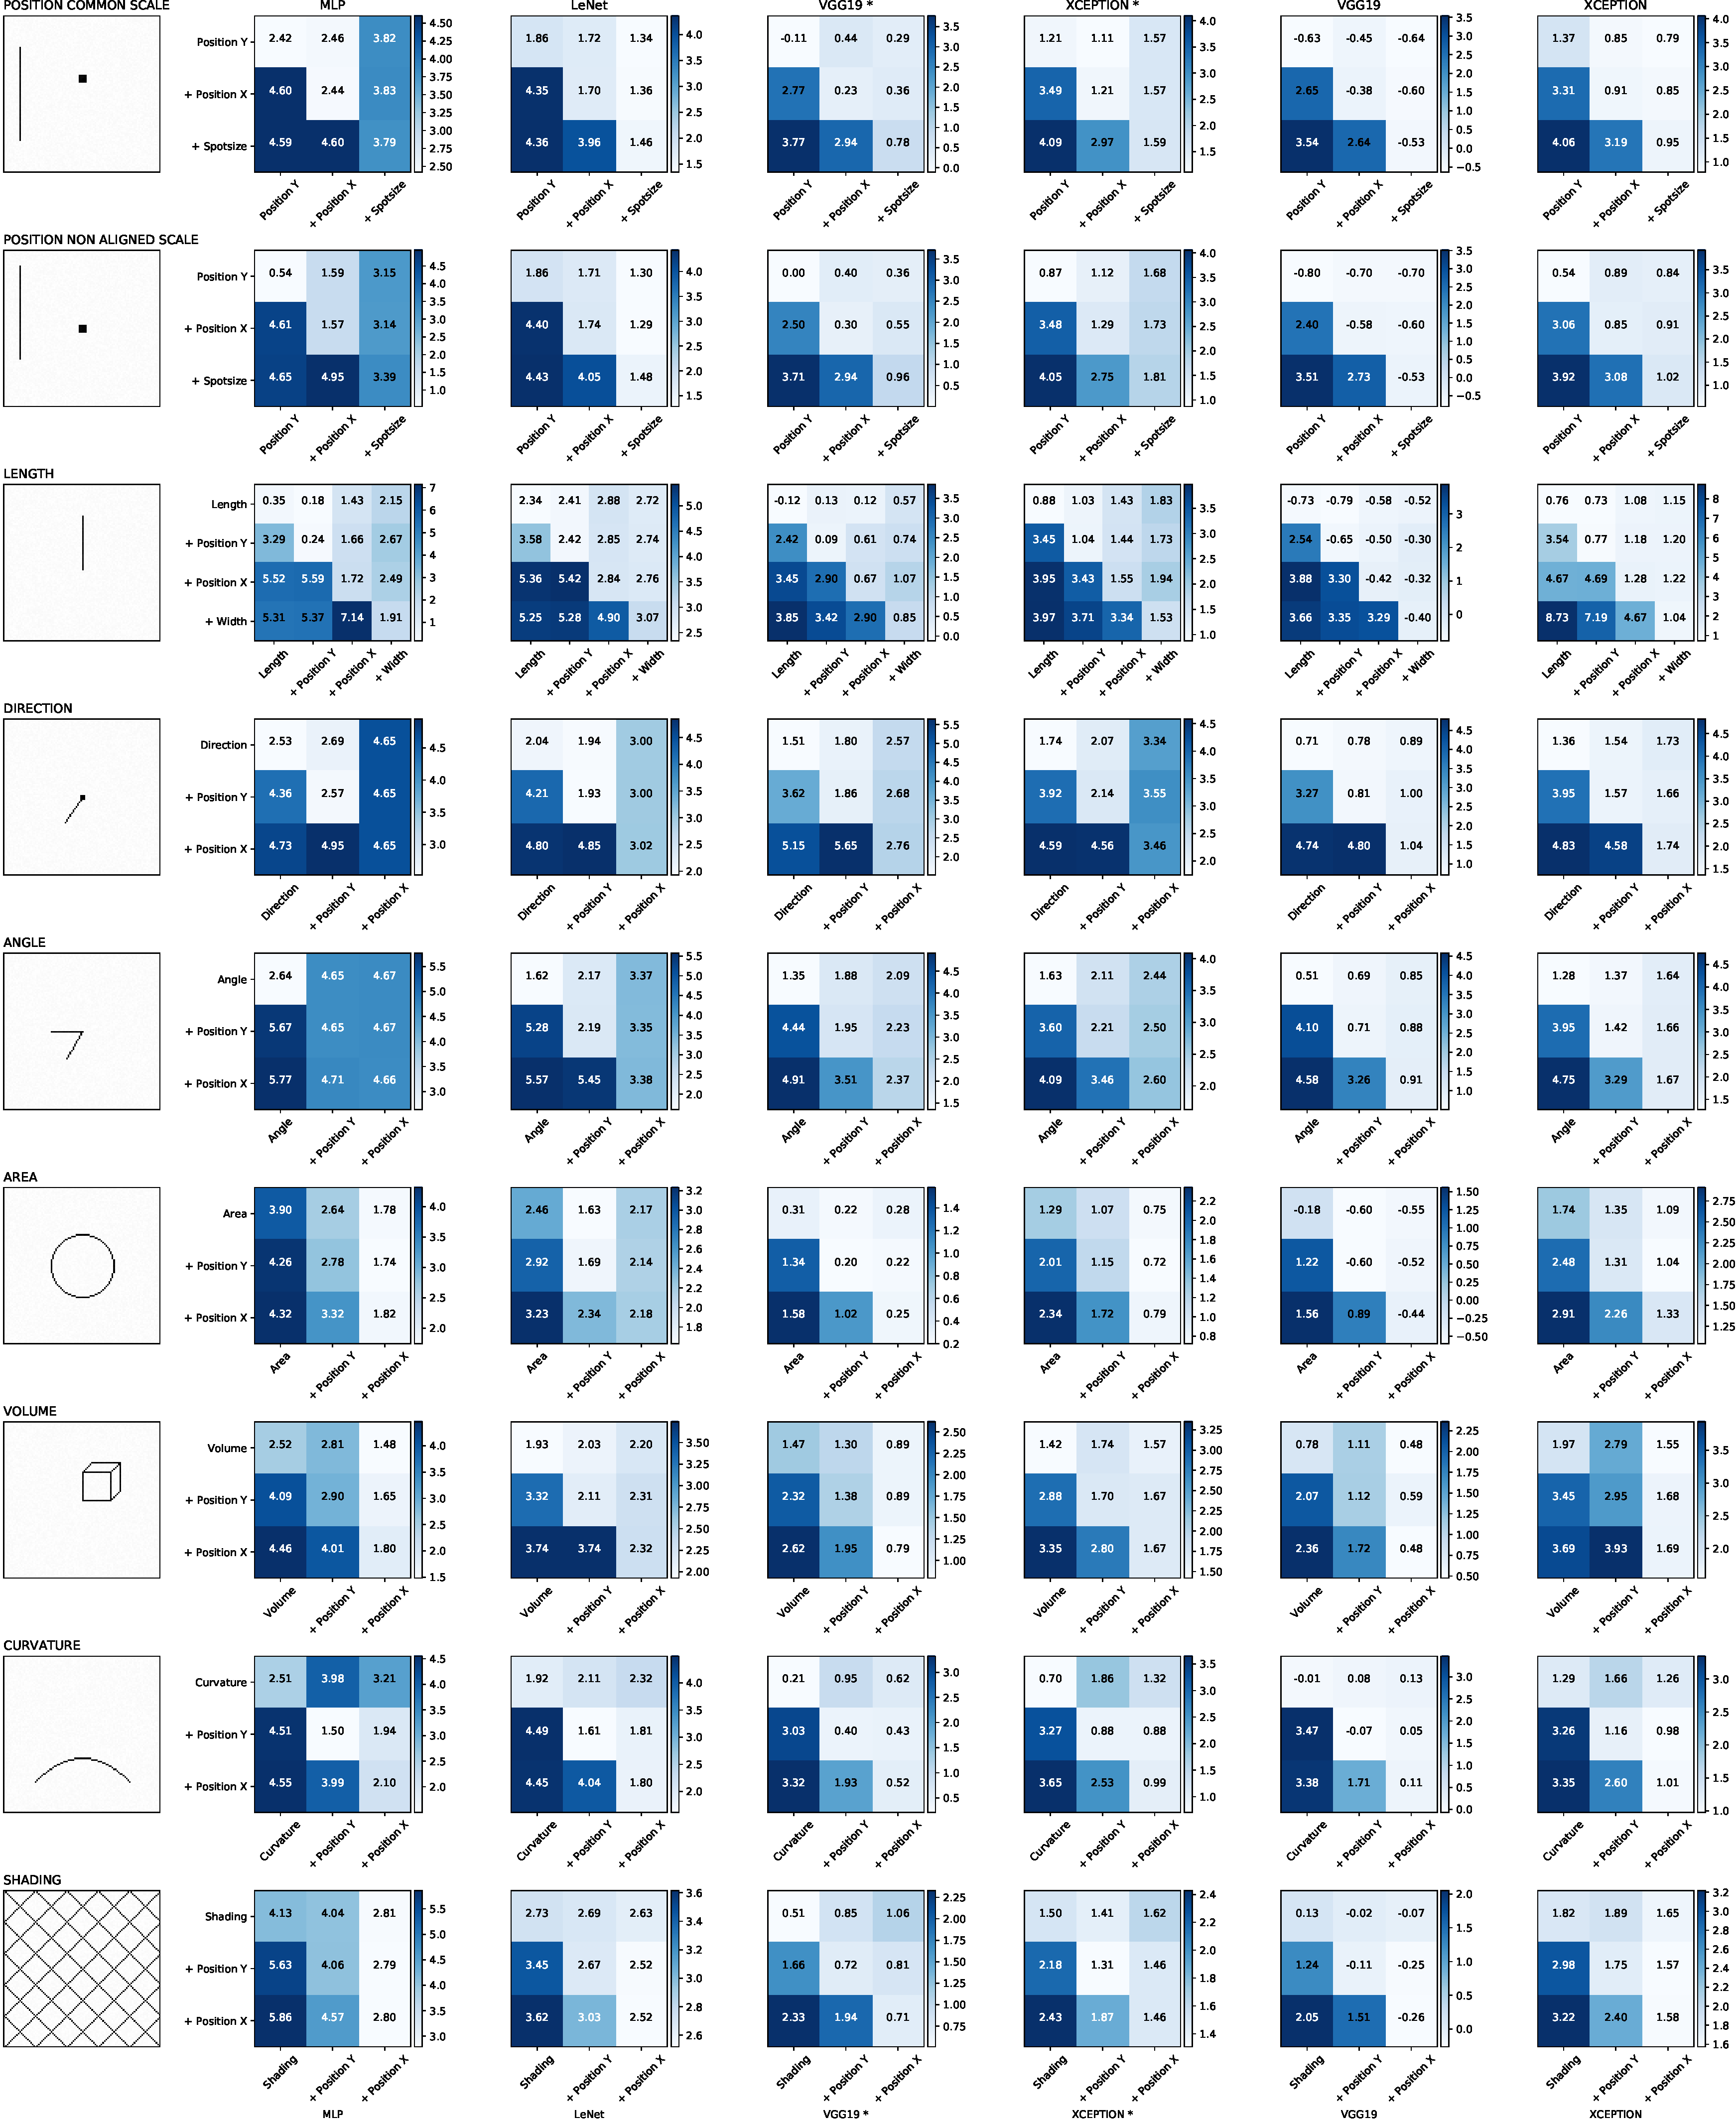
\includegraphics[width=\linewidth]{cross_network_new.pdf}
  \caption{\textbf{Cross-network variability.} Our networks fail when the stimuli changes through translation or stroke width. The x-labels indicate the training configuration while the y-labels indicate the stimuli variation. Numbers represent MLAE.}
	\label{fig:cross_network}
\end{figure*}

\begin{figure*}[p]
	\centering
	  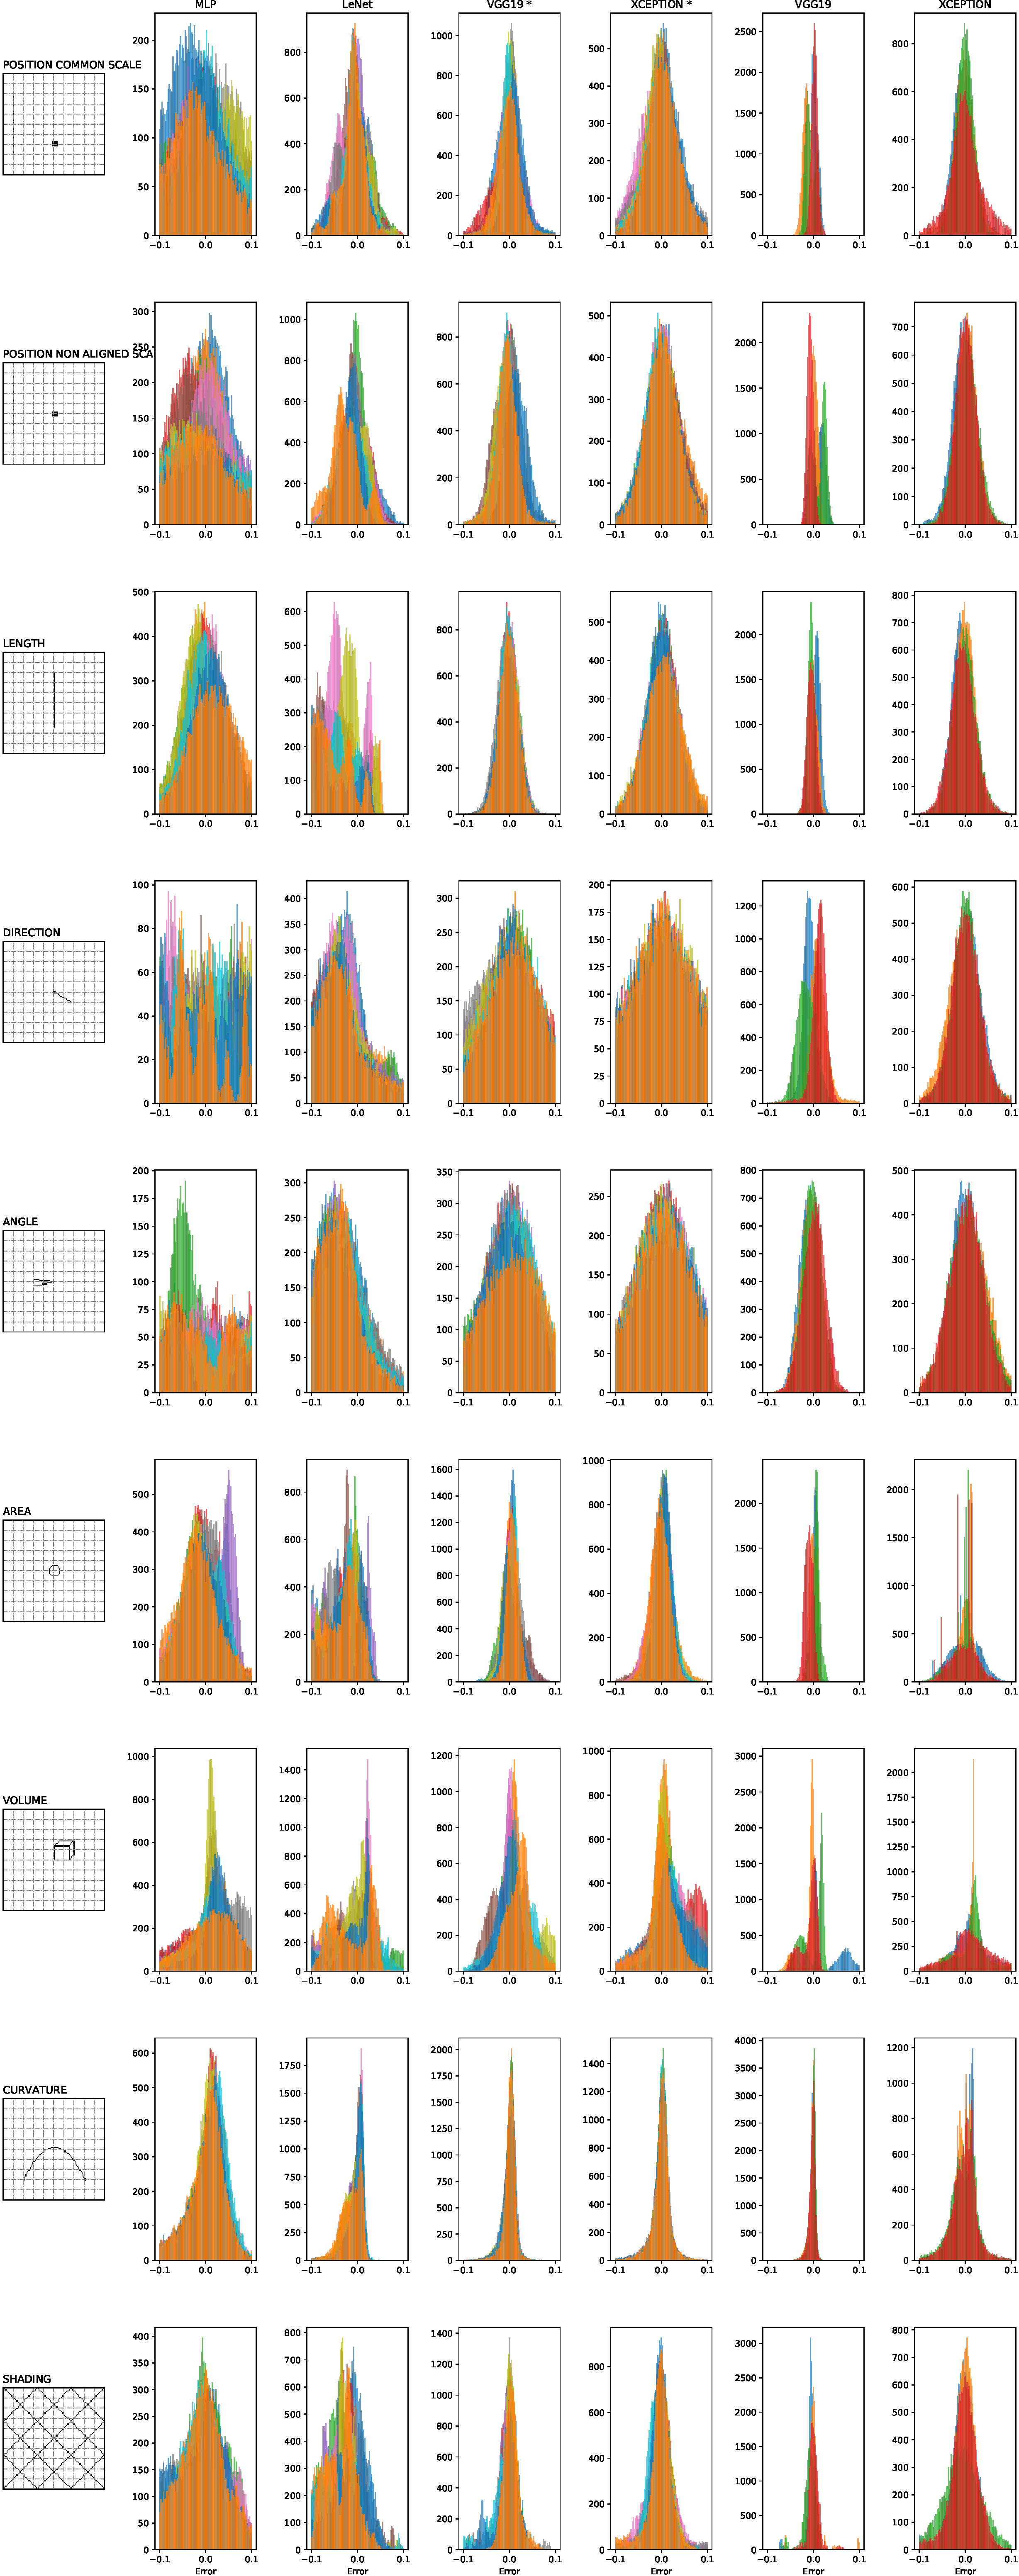
\includegraphics[width=.8\linewidth]{error_inspection_new.pdf}
  \caption{\textbf{Error distributions.} Error distributions of our networks when decoding elementary perceptual tasks.}
	\label{fig:errors}
\end{figure*}

\begin{figure}[p]
	\centering
	  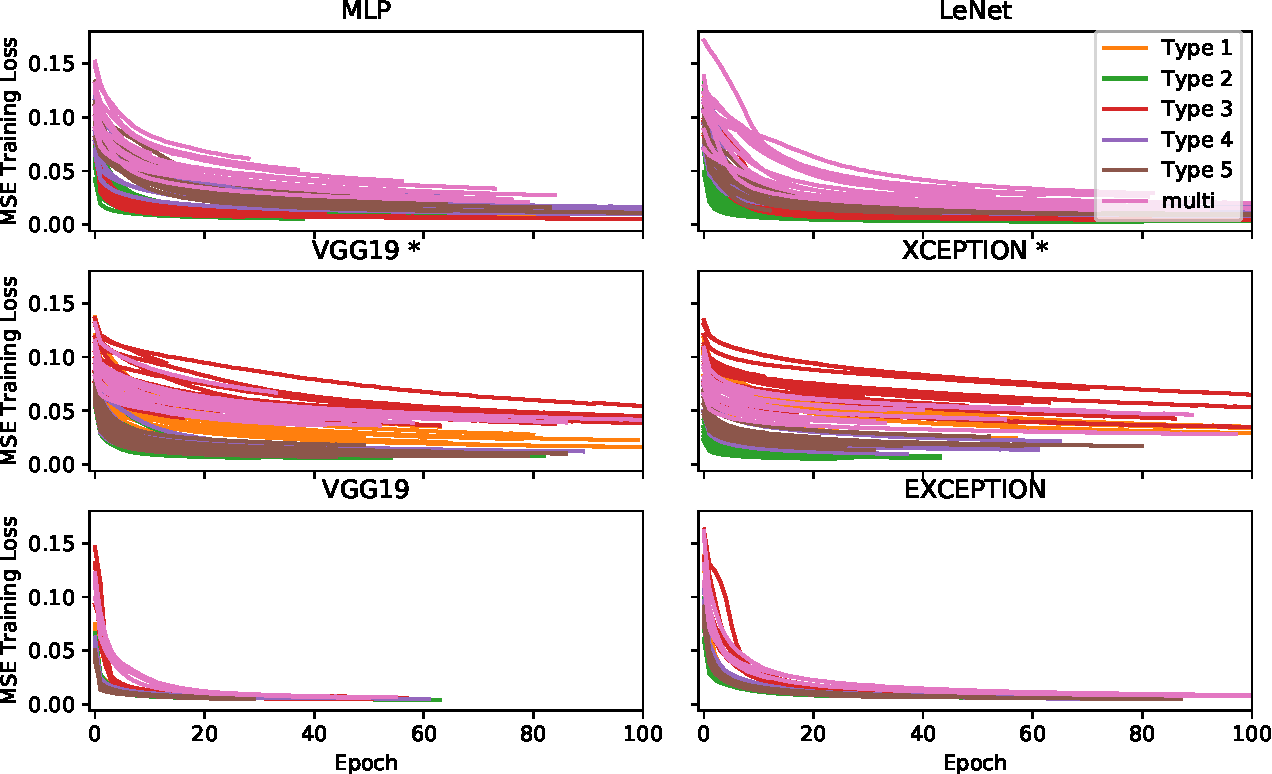
\includegraphics[width=\linewidth]{../gfx/figure4_training_loss_with_multi.pdf}
	  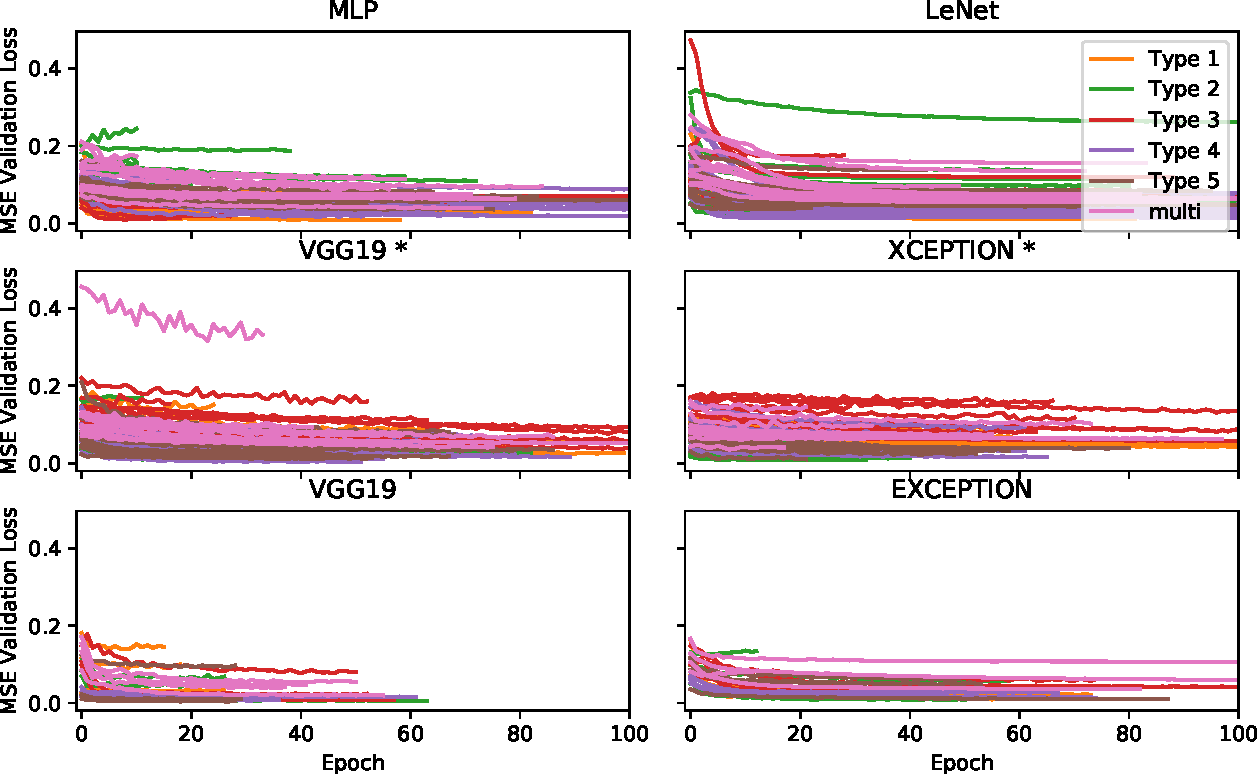
\includegraphics[width=\linewidth]{../gfx/figure4_val_loss_with_multi.pdf}
  \caption{\textbf{Loss plots for the position-length experiment.} We visualize the MSE loss on training data and for unseen validation data after each epoch. There is no significant difference in convergence for either encoding but spiky outliers due to monte-carlo cross validation are visible.}
	\label{fig:fig4_loss}
\end{figure}

\begin{figure}[p]
	\centering
	  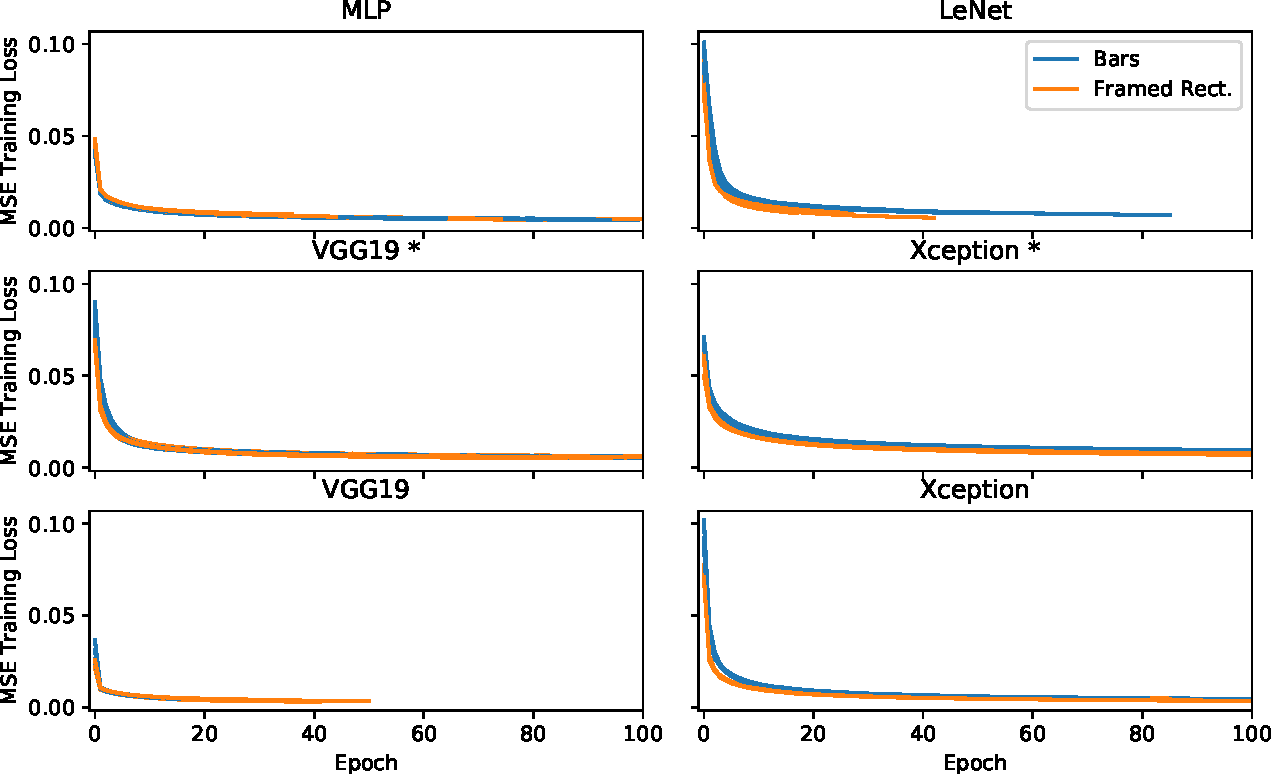
\includegraphics[width=\linewidth]{../gfx/figure12_training_loss.pdf}
	  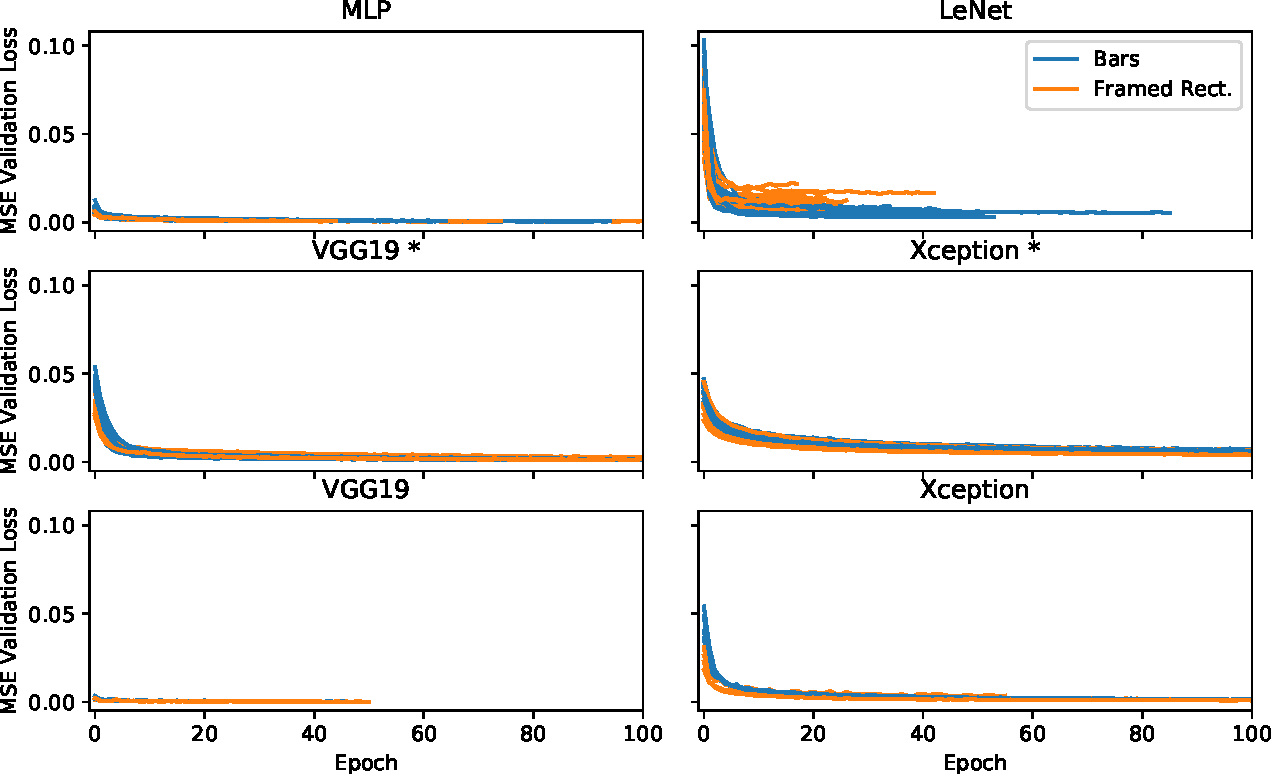
\includegraphics[width=\linewidth]{../gfx/figure12_val_loss.pdf}
  \caption{\textbf{Loss plots for the bars-and-framed-rectangles experiment.} We visualize the MSE loss on training data and for unseen validation data after each epoch. There is no significant difference in convergence for either encoding.}
	\label{fig:fig12_loss}
\end{figure}

\begin{figure*}[t]
	\centering
	
    \subfloat[without noise]{
	  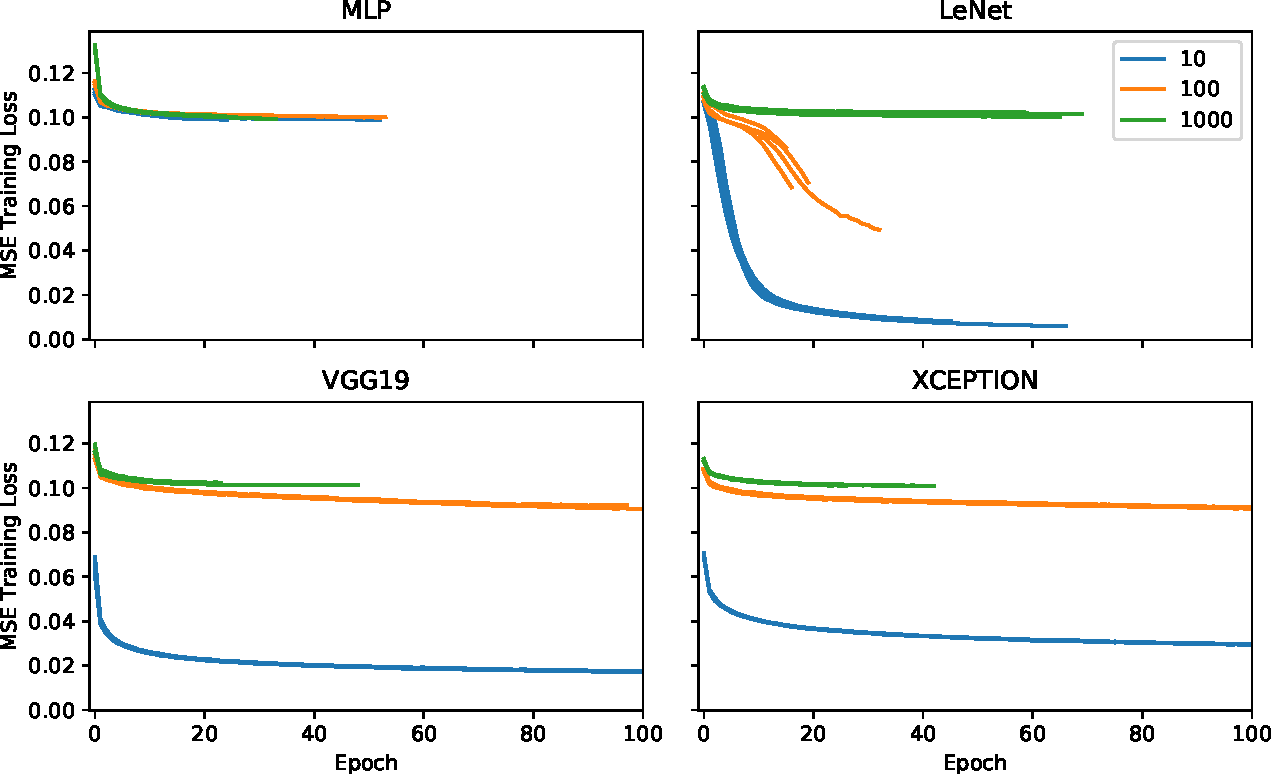
\includegraphics[width=.48\linewidth]{../gfx/weber_training_loss_no_noise.pdf}
	  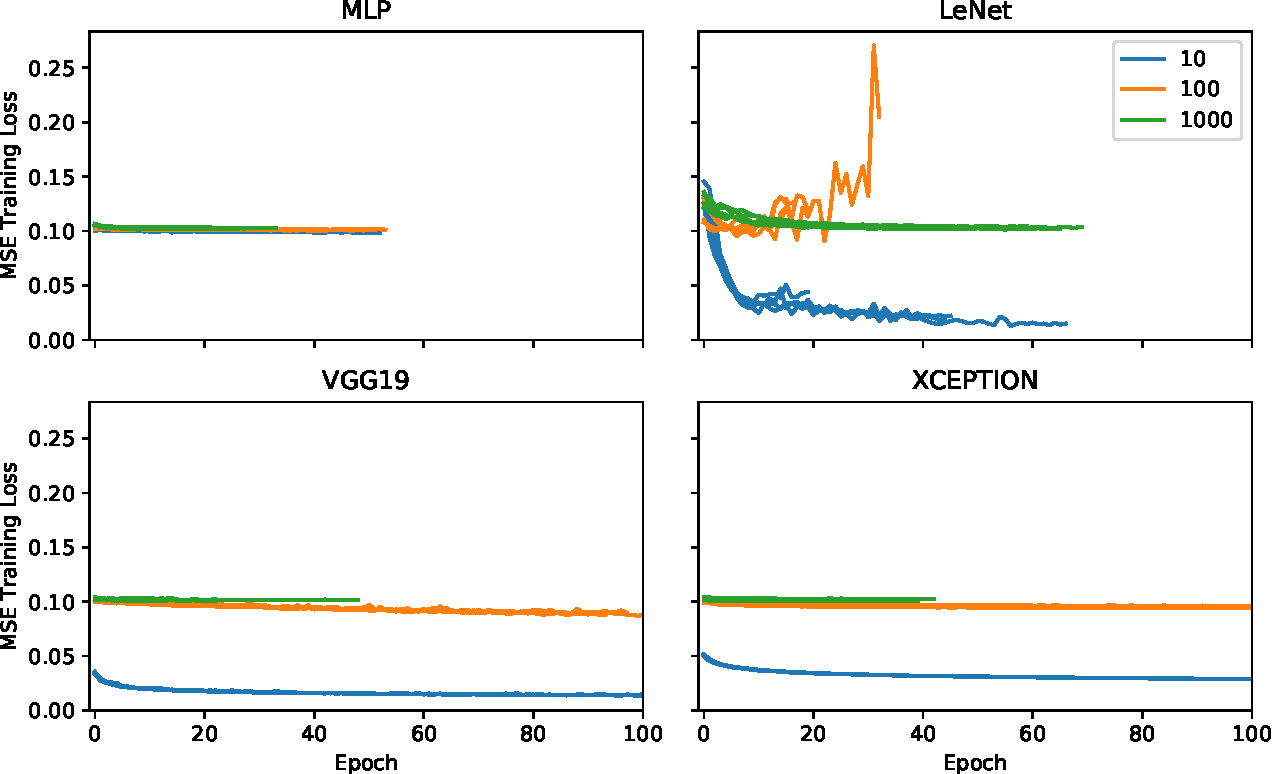
\includegraphics[width=.48\linewidth]{../gfx/weber_validation_loss_no_noise.pdf}
	}
	\hfill
    \subfloat[with noise]{
	  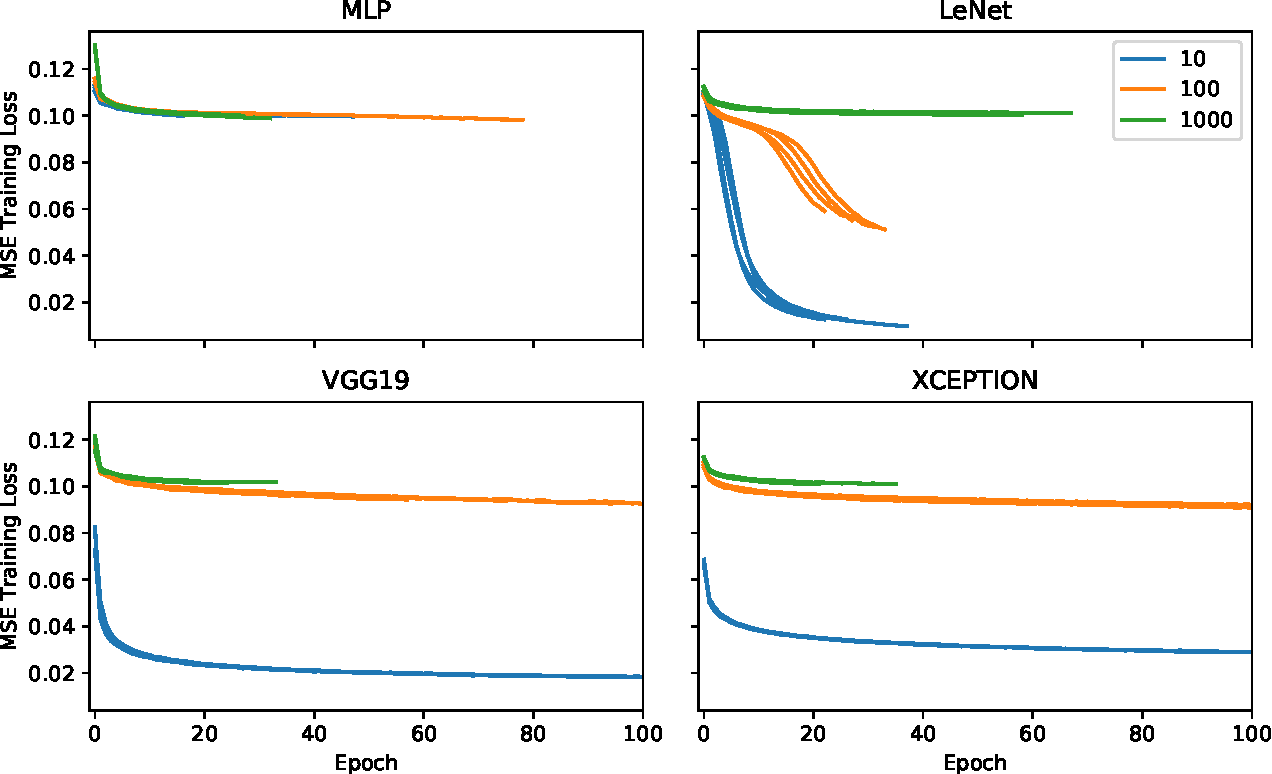
\includegraphics[width=.48\linewidth]{../gfx/weber_training_loss.pdf}
	  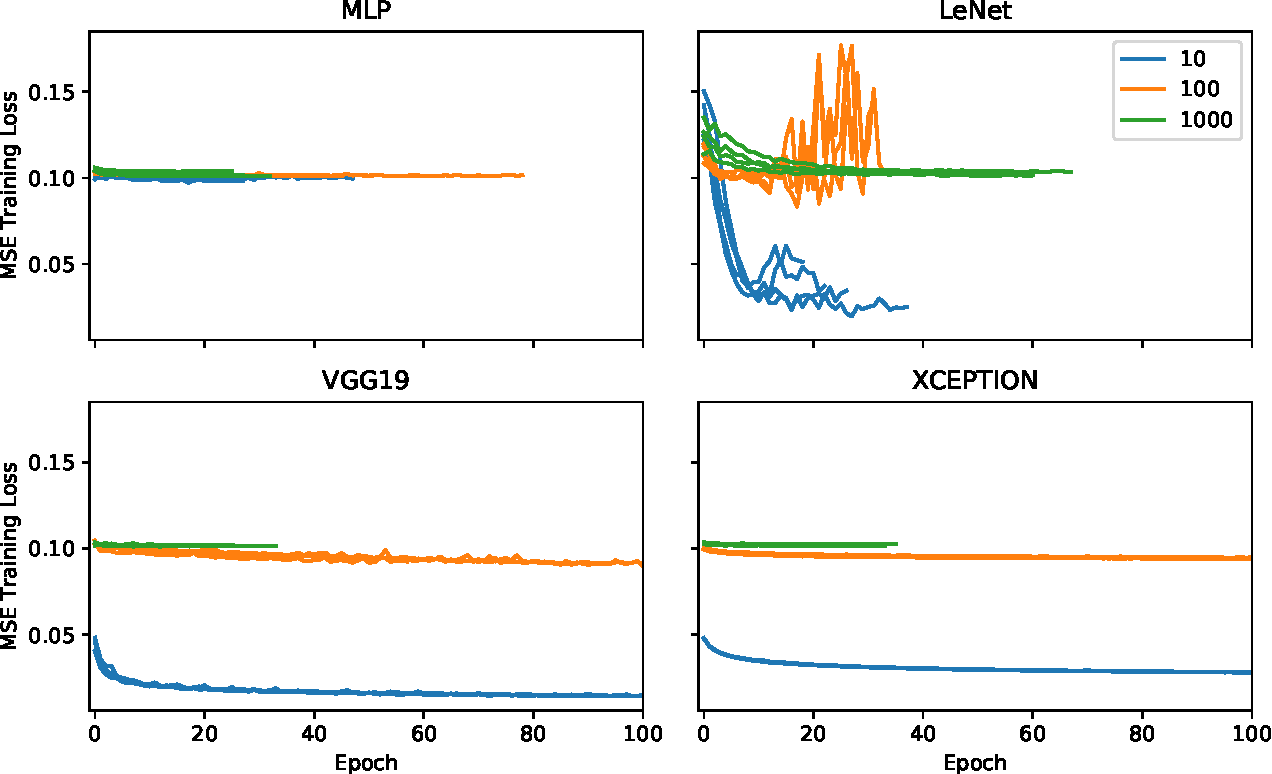
\includegraphics[width=.48\linewidth]{../gfx/weber_validation_loss.pdf}
	}

  \caption{\textbf{Loss plots for the weber-fechner's law experiment.} We visualize the MSE loss on training data (left) and for unseen validation data (right) after each epoch (a) without noise and (b) with subtle $5\%$ noise per pixel. There is no significant difference when noise is added. The LeNet network seems to overfit with Weber Base 100 in both cases even with dropout regularization.}
	\label{fig:weber_loss}
\end{figure*}

%% if specified like this the section will be committed in review mode
%\acknowledgments{
%The authors wish to thank A, B, and C. This work was supported in part by
%a grant from XYZ (\# 12345-67890).}

%\bibliographystyle{abbrv}
%\bibliographystyle{abbrv-doi}
%\bibliographystyle{abbrv-doi-narrow}
%\bibliographystyle{abbrv-doi-hyperref}
%\bibliographystyle{abbrv-doi-hyperref-narrow}

%\bibliography{../paper}
\end{document}

